%%%%%%%%%%%%%%%%%%%%%%%%%%%%%%%%%%%%%%%%%%%%%%%%%%%%%%%%%%%%%%%%%%%%%%%%%%%%%%%%
%                                                                              %
%            A Painless Introduction to Programming UAMMD Modules              %
%                                                                              %
%                          Marc Meléndez Schofield                             %
%                                                                              %
%%%%%%%%%%%%%%%%%%%%%%%%%%%%%%%%%%%%%%%%%%%%%%%%%%%%%%%%%%%%%%%%%%%%%%%%%%%%%%%%

\documentclass[a4paper,12pt,openany,hidelinks]{book}

\usepackage[hmarginratio=1:1]{geometry}
\usepackage{graphicx}
\usepackage{eso-pic}
\usepackage[utf8]{inputenc}
\usepackage{amsmath}
\usepackage{amssymb}
\usepackage{afterpage}
\usepackage{pagecolor}
\usepackage{picture}
\usepackage{comment}
\usepackage{eso-pic}
\usepackage{listings}
\lstset{language = C++,
        frame = single,
        framextopmargin = 10pt,
        morecomment = [is]{\%!}{\^^M},
        basicstyle = \footnotesize,
        breaklines=true,
        postbreak=\mbox{$\hookrightarrow$\ }}
\usepackage{hyperref}
\hypersetup{
    colorlinks,
    linkcolor={blue!50!black},
    citecolor={red!50!black},
    urlcolor={blue!80!black},
    pdftitle={A Painless Introduction to Programming UAMMD Modules},
    pdfauthor={M. Melendez},
    pdfsubject={UAMMD programming},
    pdfkeywords={molecular simulation, fluctuating hydrodynamics, UAMMD},
    pdfdisplaydoctitle
}

\begin{document}

%%%%%%%%%%%%%%%%%%%%%%%%%%%%%%%%%%%%  Head  %%%%%%%%%%%%%%%%%%%%%%%%%%%%%%%%%%%%

%%% Cover %%%

\thispagestyle{empty}
\newpagecolor{black}\afterpage{\restorepagecolor}

\AddToShipoutPicture*{
  \put(.5\paperwidth,.5\paperheight) {
    \makebox(0,0) {
      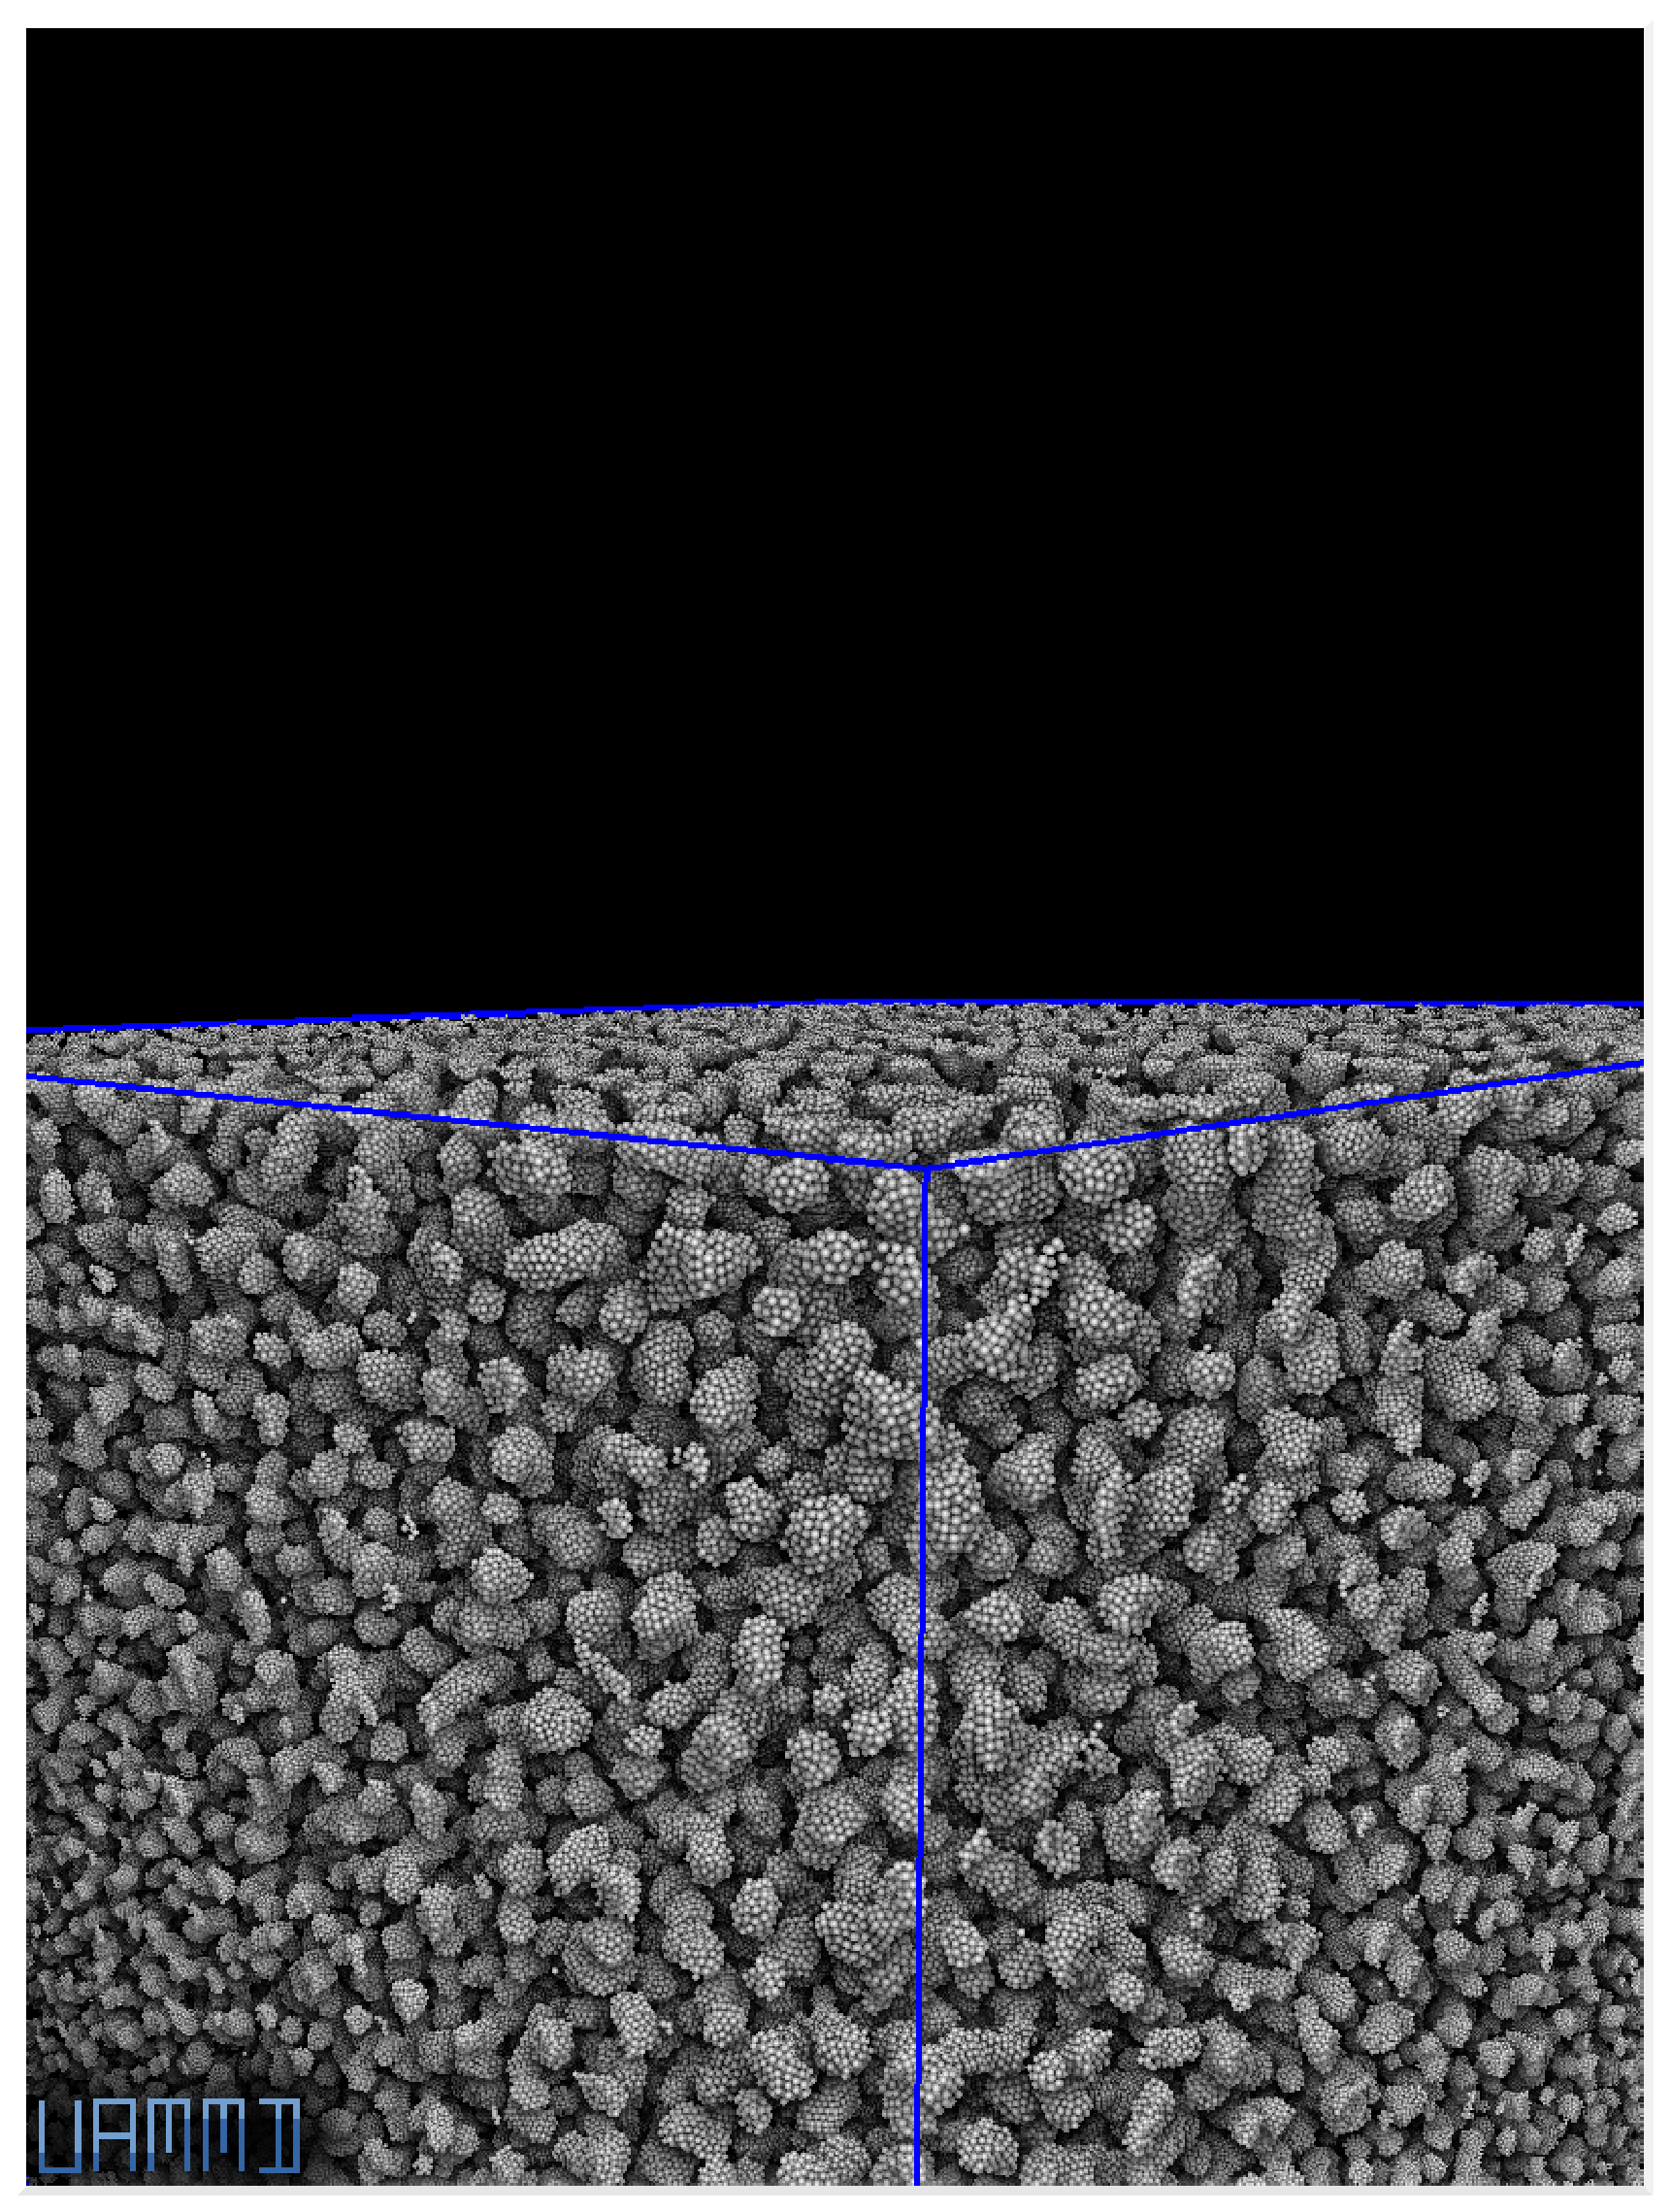
\includegraphics[width = 0.9 \paperwidth, keepaspectratio]{figures/uammd_intro_cover.eps}
    }
  }
}

\begin{center}
  {\color{white}
    \resizebox{0.8 \linewidth}{!}{\textbf{A Painless Introduction to}}

    \vspace{.5cm}

    \resizebox{\linewidth}{!}{\textbf{Programming UAMMD Modules}}
  }
\end{center}

\vspace{1.75cm}

\begin{center}
  {\huge {\color{white}Marc Mel\'endez Schofield}}
\end{center}

\vfill

\clearpage

\thispagestyle{empty}

\newgeometry{hmarginratio=2:3}


%%% Title page %%%

\title{A Painless Introduction to Programming UAMMD Modules}
\date{\today}
\author{Marc Mel\'endez Schofield}

\maketitle

%%%%%%%%%%%%%%%%%%%%%%%%%%%%%%  Copyright notice  %%%%%%%%%%%%%%%%%%%%%%%%%%%%%%


\thispagestyle{empty}


\noindent \textit{Title:} A Painless Introduction to Programming UAMMD Modules

\noindent \textit{Author:} Marc Mel\'endez Schofield. \\[1.2cm]

\vfill

\hrule

\vspace{2.0mm}

\noindent \includegraphics[height=0.75cm,clip=true]{figures/{by-nc-sa}.eps}
{\small Marc Mel\'endez Schofield (2020).} \\

{\small \noindent \textcopyright\ 2020,
Marc Mel\'endez Schofield. \textit{A Painless Introduction to Programming UAMMD
Modules} is distributed under the Creative Commons
Attribution-NonCommercial-ShareAlike 4.0 International
(\textsc{cc-by-nc-sa} 4.0). For summary and legal details visit: \\
\url{https://creativecommons.org/licenses/by-nc-sa/4.0/}}

\vspace{1cm}

\noindent \includegraphics[height=0.75cm,clip=true]{figures/{by}.eps}
{\small \textit{Cover}: Ra\'ul P\'erez Pel\'aez (2017),
 Marc Mel\'endez Schofield (2020).} \\

{\small \noindent \textit{Cover image}: \textcopyright\ 2017,
Ra\'ul P\'erez Pel\'aez. Ten million particles interacting through Lennard-Jones
potentials in a cubic periodic simulation box. Rendered with
\textit{superpunto}.

\noindent \textit{Cover design}: \textcopyright\ 2020,
Marc Mel\'endez Schofield. The cover is distributed under the Creative
Commons Attribution 4.0 International
(\textsc{cc-by} 4.0). For summary and legal details visit: \\
\url{https://creativecommons.org/licenses/by/4.0/}}

%%%%%%%%%%%%%%%%%%%%%%%%%%%%%%%%%%%%  Body  %%%%%%%%%%%%%%%%%%%%%%%%%%%%%%%%%%%%

\tableofcontents

\chapter*{Introduction}
\markboth{INTRODUCTION}{INTRODUCTION}

\section*{On UAMMD}

The \textbf{Universally Adaptable Multiscale Molecular Dynamics} project,
known as \textbf{UAMMD}, collects molecular simulation algorithms for Graphics 
Processing Units (GPUs) into header-only code. In layman's terms, this means 
that you can write programs in CUDA and include high-performance algorithms to 
carry out rigorous classical dynamics many-body simulations. UAMMD relies on the 
GPU's capacity to perform huge amounts of analogous computations in parallel to 
increase the speed at which it works out many-body interactions.

The program was written mostly by Ra\'ul P\'erez Pel\'aez as a PhD candidate at
UAM, in Madrid. As a consequence, it became strongly focused on the interests of
the author. If you would like to use UAMMD to carry out some particular type of
simulation like, say, ReaxFF molecular dynamics, then you will probably have to
code it yourself. However, he did implement some very advanced modules for
fluctuating hydrodynamics so, if your research lies on that path, you will
definitely want to check out UAMMD. In my view, the great strength of UAMMD
comes from the abstract methods it provides to deal with many-body interactions
on the GPU, allowing you to quickly write simple but extremely efficient
simulations.

%! codeblock: OnUAMMD
As the title of this book states, I aim to provide you with a painless 
introduction to writing UAMMD modules. I am writing with our research group's 
students in mind, imagining that you have begun to learn about molecular
simulation and have some (but not much) background in physics and programming.
If you need a more advanced approach, refer to the Wiki pages on the UAMMD
repository. Even if you don't, but you feel a painfully slow progress reading
this book, please skim through the pages and skip ahead until you find an
interesting section.
%! codeblockend

\section*{Beginner C++}

This section would be a good example of a chunk of text that you can skip and 
still be fine, as long as you have some very basic knowledge of what a C or C++ 
program looks like. The point here is \textit{not} to teach you C++, but rather 
to give you some basic feel for the language allowing you to read on and 
understand the gist of the code boxes. That should be enough for experimenting 
by tweaking the examples given here. You will, of course, eventually have to 
learn some CUDA if you wish to write advanced UAMMD programs, but there is a 
whole sea of free online resources out there. Instead of sailing out, it might 
be a good idea to understand what you want to know first (if your desires draw 
you out to sea, by all means go forth and sail!).

Below, I have copied the iconic ``Hello, World'' program, written for C++. It
begins by including input/output functionality by adding the \texttt{iostream}
standard library to our program (\texttt{iostream} contains \texttt{cout} and
texttt{endl} used a few lines down). We then specify that we will be using
the standard (txttt{std}) versions of \texttt{cout} and \texttt{endl}, which
saves us from having to write \texttt{std::cout} or \texttt{std::endl} each
time we want to mention them.
\begin{lstlisting}
%! codefile: code/helloWorld.cpp
# include <iostream>

using std::cout;
using std::endl;

%! codeinsert: functionDefinitions
int main(int argc, char * argv[])
{
  cout<<"Hello, World!"<<endl;
  %! codeinsert: multiplesOfThree
  %! codeinsert: functionCalls
	return 0;
}
%! codeend
\end{lstlisting}

The final lines of code implement the \texttt{main} function. C++ programs
always execute this function first.

To define a function, we write the return value first, then the function name
followed by a list of arguments in parentheses. The contents come after the
arguments, so functions look like this:
\begin{lstlisting}
returnvalue functionname(list, of, arguments)
{
  what the function does
}
%!
\end{lstlisting}

Our ``Hello, World'' \texttt{main} function returns an integer (\texttt{int})
value: zero, in fact. As you can see, the function ends with \texttt{return 0;}.
Note that instructions end with a semicolon (;). The main function arguments, an
integer called \texttt{argc} and an array of strings called \texttt{argv}, refer
to the number of command-line arguments and the arguments themselves with which
the program was executed. In the next chapter, we will be passing these values
on to a UAMMD function that will deal with them. Here, we just ignore them.

The remaining line directs the ``\texttt{Hello, World!}'' string to standard
output, so that it would typically be printed on the screen, followed by an
end of line.

Compile the code above with \texttt{g++ helloWorld.cpp -o helloWorld}, or
something similar. Running the program should print ``Hello, World!'' on the
screen.

The compiler ignores anything you write between \texttt{/*} and \texttt{*/}, so
you can use these characters to insert explanatory comments in your code. In a
typicaly program, you will declare variables, data structures and classes, on
which you will later carry out some calculations. UAMMD code might include lines
like these.
\begin{lstlisting}
int numberOfParticles; /* An integer value */
real temperature; /* A floating-point real value */
Box simulationBox(10); /* A cubic box of side 10 units */
bool printPositions; /* A boolean (true or false) value */
%!
\end{lstlisting}

We will control program flow with \texttt{for} and \texttt{if}. A \texttt{for}
loop like
\begin{lstlisting}
  for(int i = 1; i <= 100; ++i) {
    cout<<"Iteration: "<<i<<endl;
  }
%!
\end{lstlisting}
will begin by setting the integer \texttt{i} equal to 1. It will then execute
the \texttt{cout} code on the line below time and again while \texttt{i} does
not exceed \texttt{100}. After each iteration of the code, it will increase the
variable \texttt{i} by one (this is what \texttt{++i} does). Each time, it
prints out ``\texttt{Iteration:}'', followed by the value of \texttt{i}.

When you want the program to do something different depending on whether 
something else happened, you typically write code with the following structure.
\begin{lstlisting}
  if(this_is_true) {
    then_do_this();
    and_this();
  }
%!
\end{lstlisting}
Sometimes you want to specify what the program should do otherwise by adding
\begin{lstlisting}
  else {
    do_this_instead();
  }
%!
\end{lstlisting}
For example, suppose we wanted to print the number only every thirteen steps,
then we would replace the content of the for loop like this.
\begin{lstlisting}
%! codeblock: multiplesOfThree
  int printEverynSteps = 13;

  for(int i = 1; i <= 100; ++i) {
    if(printEverynSteps > 0
       && i % printEverynSteps == 0) {
        cout<<"Iteration: "<<i<<endl;
    }
  }
%! codeblockend
\end{lstlisting}
The \texttt{if} block says that if \texttt{printEverynSteps} is a positive 
number (\texttt{> 0}) and (\texttt{\&\&}) the remainder of the step number
divided by \texttt{printEverynSteps} equals zero (\texttt{step \%
printEverynSteps == 0}), then the line is printed. Compiling and
running the program outputs:
\begin{lstlisting}
Hello, World!
Iteration: 13
Iteration: 26
Iteration: 39
Iteration: 52
Iteration: 65
Iteration: 78
Iteration: 91
%!
\end{lstlisting}

Much of UAMMD code will be calling functions or methods defined elsewhere.
Let us add the following two functions before \texttt{main}.
\begin{lstlisting}
%! codeblock: functionDefinitions
int add(int a, int b) {
  return a + b;
}

void goodbye() {
  cout<<"Goodbye!"<<endl;
  return;
}
%! codeblockend
\end{lstlisting}
The first function takes two integers and returs their sum. The second takes no
arguments and returns none, but prints out ``Goodbye!''. To call these functions
after the \texttt{for} loop in our code, we simpy give their names followed by
their arguments in parentheses.
\begin{lstlisting}
%! codeblock: functionCalls
  cout<<"3 + 5 = "<<add(3,5)<<endl;
  goodbye();
%! codeblockend
\end{lstlisting}

\section*{\label{basic_simulation}Simulating classical particle physics}
\label{basic_simulation}

Numerical simulations of physical systems made up of particles usually involve
four steps.
\begin{enumerate}
  \item Declare the variables representing the state of the system.
  \item Set the variables to their initial values.
  \item Calculate how the system evolves in time by integrating the
        equations of motion, dealing with how each particle interacts with its
        environment.
  \item Print out final results and clean up.
\end{enumerate}

As an easy illustration, let us write a program for a bouncing rubber ball We 
begin by defining the simulation variables and parameters. Newton's second law 
tells us that the ball's acceleration $\mathbf{a}$ (which is the second 
derivative of the position $\mathbf{r}$ with respect to time) equals the 
acceleration of gravity.
\begin{equation*}
  \mathbf{a} = \frac{d^2\mathbf{r}}{dt^2} = \mathbf{g}.
\end{equation*}
Now, $\mathbf{g}$ equals $-9.8\ \mathrm{m/s}^2$ in the vertical direction. To
calculate the motion of the ball, we track the change in its position and
velocity in small increments of size \texttt{dt}. At every step, we change the
velocity by adding a change of $-9.8\ dt$ in the vertical direction and then
update the position by moving the ball to a new position using its current
velocity. Given $\mathbf{r}(n)$ and $\mathbf{v}(n)$, the position and velocity
at time step number $n$, we calculate the new position and velocity as
\begin{align*}
  \mathbf{r}(n) & = \mathbf{r}(n) + \mathbf{v}(n)\ dt, \\
  \mathbf{v}(n) & = \mathbf{v}(n) + \mathbf{g}\ dt.
\end{align*}
This simple numerical integration algorithm is known as the \textit{Euler
scheme}.

In our code, we will have to track the horizontal and vertical components of
the position and velocity, which we store in the two-dimensional arrays
\texttt{r[2]} and \texttt{v[2]}: \texttt{r[0]} will represent the horizontal
coordinate and \texttt{r[1]} the vertical component, and similarly for
\texttt{v[0]} and \texttt{v[1]}. Next, we will indicate the number of steps to
calculate, the size of the time step and how often to print out the position.
\begin{lstlisting}
%! codefile: code/rubberBall.cpp
# include <iostream>

using std::cout;
using std::endl;

int main(int argc, char * argv[])
{
  /* State of the rubber ball */
  float r[2]; /* Position (measured in metres) */
  float v[2]; /* Velocity (in metres/second) */

  float g = -9.8; /* Acceleration of gravity (in m/s^2) */

  /* Integration parameters */
  int nsteps = 10000; /* Number of time steps to calculate */
  float dt = 0.001; /* Size of time step (in seconds) */
  int printEverynSteps = 20;
%! codepause
\end{lstlisting}
The second step on our list suggests that we specify the initial conditions.
\begin{lstlisting}
%! codecontinue: code/rubberBall.cpp
  /* Initial conditions */
  r[0] = 0;
  r[1] = 2;
  v[0] = 0.5;
  v[1] = 1;
%! codepause
\end{lstlisting}
Thirdly, we integrate the equations of motion with Euler's algorithm. When we
update the positions and velocities, we must take into account collisions with
the floor. If the ball hits the floor, the vertical component of its velocity
reverses and it looses some of its momentum. At the end of the \texttt{for}
loop we print out one in every 10 steps.
\begin{lstlisting}
%! codecontinue: code/rubberBall.cpp
  /* Euler integration of the equations of motion */
  for(int step = 0; step <= nsteps; ++step) {
    /* New position */
    r[0] = r[0] + v[0]*dt;
    r[1] = r[1] + v[1]*dt;

    /* New velocity */
    v[1] = v[1] + g*dt;

    /* Deal with collisions */
    if(r[1] <= 0 && v[1] < 0) {
      v[0] = 0.9*v[0];
      v[1] = -0.8*v[1];
    }

    /* Output state */
    if(printEverynSteps > 0
       && step % printEverynSteps == 0) {
      cout<<step*dt<<" "<<r[0]<<" "<<r[1]<<endl;
    }
  }
%! codeend
\end{lstlisting}
Finally, we close down the program.
\begin{lstlisting}
%! codecontinue: code/rubberBall.cpp
  cout<<"# Simulated time: "<<nsteps*dt<<" seconds. #"<<endl;
  return 0;
}
%! codeend
\end{lstlisting}
Compiling and running the code generated the data used to plot the trajectory
in Fig. \ref{rubberBall}.

\begin{figure}
  \centering
  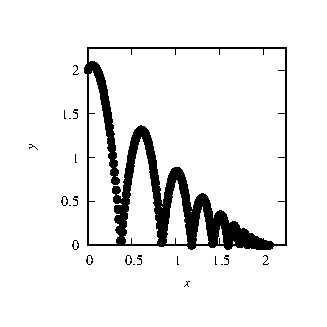
\includegraphics[width = 0.65 \textwidth]{figures/rubberBall.eps}
  \caption{\label{rubberBall}Trajectory of a bouncing rubber ball calculated
           with the code written in the previous pages.}
\end{figure}


\section*{Installing CUDA}

To make UAMMD programs, you will need to install a CUDA compiler and you will
have to run the programs on a compatible GPU device. Saying more would lead us
too far astray into a land that I do not wish to visit, so I recommend you check
the documentation for UAMMD and CUDA.


\chapter{Our first UAMMD simulation}

%%%%%%%%%%%%%%%%%%%%%%%%%%%%%%%%%%%%%%%%%%%%%%%%%%%%%%%%%%%%%%%%%%%%%%%%%%%%%%%%
%                                                                              %
%            A Painless Introduction to Programming UAMMD Modules              %
%                    Chapter 1: Our first UAMMD simulation                     %
%                                                                              %
%                          Marc Meléndez Schofield                             %
%                                                                              %
%%%%%%%%%%%%%%%%%%%%%%%%%%%%%%%%%%%%%%%%%%%%%%%%%%%%%%%%%%%%%%%%%%%%%%%%%%%%%%%%

Let us take the first step of our journey towards high-performance computing on
GPUs with a low-performance simple program that does hardly no computing. We
will modify a typical ``Hello, World!'' program in C++ slightly by adding a few
more lines (marked below with the comment \texttt{/* UAMMD */}). Note that we
also included the \texttt{using std::make\_shared} line so that we can later
declare \texttt{System} as a shared pointer (if you do not know what this means,
it doesn't matter right now).
\begin{lstlisting}
%! codefile: code/minimal.cu
# include <iostream>
# include "uammd.cuh" /* UAMMD */

using namespace uammd; /* UAMMD */
using std::make_shared;
using std::endl;
using std::cout;

int main(int argc, char *argv[]){

  auto sys = make_shared<System>(argc,argv); /* UAMMD */

  cout<<endl<<"--> Hello, UAMMD! <--"<<endl<<endl;

  sys->finish(); /* UAMMD */

  return 0;
}//!
%! codeend !//
\end{lstlisting}
Compile the code with
\begin{verbatim}
nvcc -O3 -I../uammd/src -I../uammd/src/third_party -o minimal
minimal.cu
\end{verbatim}
making sure that you replace the paths to UAMMD src code with the right path on
your system. With luck, the program will compile without problems. If it does
not, check the instructions for your system and the compiling information at the
UAMMD repository.

Running \texttt{./minimal} outputs some UAMMD information, with your ``Hello, 
UAMMD!'' message in the middle. Take out all the lines marked \texttt{/* UAMMD 
*/} and you are left with a typical ``Hello, World!'' program in C++ that only 
outputs your message.

It might be helpful to go through the program to explain what each UAMMD line 
does in very general terms. You \texttt{include} the \texttt{uammd.cuh} header 
file and use the \texttt{uammd} namespace to have access to the functionality 
defined in the UAMMD source code. Within the main function, we enclose all our 
UAMMD code between the creation of a \texttt{System} and its \texttt{finish}
call. The \texttt{System} represents the computing environment in UAMMD. It
deals with access to the GPU and random number generation on the CPU, for
example. In the code above, we created a \texttt{System} named \texttt{sys} with
\begin{verbatim}
auto sys = make_shared<System>(argc,argv);
\end{verbatim}
and called \texttt{sys->finish()} at the end of the program to ensure a graceful
exit.

The program compiles and runs, but it feels like an empty sandwich. By expanding
it slightly, though, we can run a simple simulation.

\section{\label{physical_system}The physical system}

The main sandwich filling in our virtual kitchen has to be the physical system
that we wish to simulate, represented as a collection of particles. Define them
with the following lines after declaring \texttt{sys}.
\begin{lstlisting}
%! codeblock: particleData
  int numberOfParticles = 100000;
  auto particles
    = make_shared<ParticleData>(numberOfParticles, sys);//!
%! codeblockend !//
\end{lstlisting}
From now on, we have access to all the properties of our particles. We might, 
for example, decide to distribute the particles randomly within an imaginary 
128-unit box. In the following snippet, a code block set apart by brackets
defines \texttt{position} as a local variable, meaning that it cannot be
accessed from  other parts of the code, in contrast to \texttt{L}. Let it
replace the ``Hello, UAMMD!'' line above.\label{initialConditions}
\begin{lstlisting}
%! codeblock: initialConditions
  real L = 128;
  %! codeinsert: simulationBox

  {
    auto position
      = particles->getPos(access::location::cpu,
                          access::mode::write);

    for(int i = 0; i < numberOfParticles; ++i)
      position[i]
        = make_real4(sys->rng().uniform3(-0.5, 0.5), 0)*L;
  }//!
%! codeblockend !//
\end{lstlisting}
In the \texttt{for} loop we go over the list of positions and assign to each of
them a random four-dimensional vector. The first three components are random
numbers chosen from a uniform distribution between $-0.5$ and $0.5$ the last one
is zero. Because we then multiply the vector by \texttt{L}, we finally get
coordinates in the $-\frac{L}{2}$ to $\frac{L}{2}$ range. \texttt{L} was defined
as a \texttt{real} value. Depending on the options at compilation, this means
either a floating point or a double precision number. The final number in the
four-vector represents the particle type (here set to zero).

Making the position variable local guarantees that we will not try to read it
later on, thinking that we have access to the positions, but without having
received the updated values. Use \texttt{getPos} every time you need to access
the positions.

Suppose that, instead of writing to the particle positions, we wished to read
the velocities. The code snippet would resemble the box above, but we would call
\texttt{getVel} instead of \texttt{getPos} and indicate that we wish to read the
values.
\begin{lstlisting}
    auto velocities
      = particles->getVel(access::location::cpu,
                          access::mode::read);
\end{lstlisting}
Other particle properties work similarly: use \texttt{getMass},
\texttt{getRadius}, \texttt{getCharge}, \texttt{getForce} or \texttt{getEnergy}.

Each particle is born with a name or identification number, which you may think
of as a serial number, accessible with the \texttt{getId} method. The reason why
you should care about this name concerns UAMMD reshuffling all the particles
every once in a while for efficiency. If you wish to track the trajectory of the
particle pointed at by \texttt{positions[3]}, you must remember that later on in
the code, when you get the positions with \texttt{getPos}, \texttt{positions[3]}
might be pointing at the location of a different particle.

Generally speaking, you will want to traverse the particle data in the order
provided by these \texttt{getWhatever} functions when you want to perform an
operation on all the particles, but don't care about the order, like when you
calculate the force on each particle. If you wish to track trajectories, for
example, then you need to identify the particles by name. So, if you would
like to print out the positions in the same order every time, use this:

\label{particlePositions}
\begin{lstlisting}
      auto position
        = particles->getPos(access::location::cpu,
                            access::mode::read);
      const int * index = particles->getIdOrderedIndices(access::location::cpu);

      out<<endl;
      for(int id = 0; id < numberOfParticles; ++id)
        out<<position[index[id]]<<endl;
\end{lstlisting}
After getting the positions, you get a list of the indices ordered by name. Say
that you are searching for a particle with \texttt{id = 3}. Then
\texttt{index[id]} would tell you where it lies in the particle list, and
\texttt{position[index[id]]} would give you its position in space (and its type
as the fourth component of the position vector).

\section{Integrating the equations of motion}

The next ingredients adding flavour to our sandwich are time and motion. To get
the particles to move, we have to integrate their equations of motion
numerically. Now, we keep the new feature as simple as possible by assuming that
the particles do not interact, and treat them as atoms in an ideal gas.

We need some more functionality, which we import into our project with
\begin{lstlisting}
# include "Integrator/VerletNVE.cuh"
\end{lstlisting}
at the beginning of the file, after including the \texttt{uammd.cuh} header 
file. Now we can use the Verlet scheme to integrate the equations of motion, but 
we need to set the values of some parameters first. The \texttt{dt} element sets 
the size of the integration time step. In the introduction, we used Euler's 
algorithm to carry out the integration, but Verlet came up with a very popular 
method which improved the accuracy of integration at very little extra 
computational cost. We will choose his method here.
\begin{lstlisting}
%! codeblock: VerletParams
  using Verlet = VerletNVE;
  Verlet::Parameters VerletParams;
  VerletParams.dt = 0.01;
  VerletParams.initVelocities = true;
  VerletParams.energy = 1.0;//!
%! codeblockend !//
\end{lstlisting}
In addition, we use the algorithm to initialise the velocities to random values
in such a way that the energy per particle equals \texttt{1.0}. Having set the
parameters, we activate the integrator with the following line.
\begin{lstlisting}
%! codeblock: Verlet
  auto integrator
    = make_shared<Verlet>(particles, sys, VerletParams);//!
%! codeblockend !//
\end{lstlisting}

Leaving their initial random positions, we allow the atoms to drift away. The 
program, we decide, will write the positions to \texttt{free\_expansion.dat}.
\begin{lstlisting}
%! codeblock: outputFile
  std::string outputFile = "freeExpansion.dat";
  std::ofstream out(outputFile);

  int numberOfSteps = 1000;
  int printEverynSteps = 100; //!
%! codeblockend !//
\end{lstlisting}
Although we will tell the computer to calculate one thousand time steps, we
will only record the state of the system once every one hundred steps. 

To advance the system in time, use the integrator's \texttt{forwardTime} method.
\begin{lstlisting}
%! codeblock: integration
  for(int step = 0; step < numberOfSteps; ++step) {
    integrator->forwardTime();

    if(printEverynSteps > 0
       and step % printEverynSteps == 1) {
      /* ... Output particle positions ... */
      %! codeinsert: printPositions
    }
  } //!
%! codeblockend !//
\end{lstlisting}
You can easily replace the comment above with the output code explained at the
end of section \ref{physical_system} (page \pageref{particlePositions}).

\begin{comment}
\begin{lstlisting}
%! codefile: code/freeExpansion.cu
# include <iostream>
# include "uammd.cuh"
# include "Integrator/VerletNVE.cuh"

using namespace uammd;
using std::make_shared;
using std::endl;

int main(int argc, char *argv[]){

  auto sys = make_shared<System>(argc, argv);

  %! codeinsert: particleData

  %! codeinsert: initialConditions

  %! codeinsert: VerletParams

  %! codeinsert: Verlet

  %! codeinsert: outputFile

  %! codeinsert: integration

  sys->finish();

  return 0;
} //!
%! codeend !//
\end{lstlisting}
\end{comment}

We should now have a working, admittedly unexciting, simulation. It represents 
the free expansion of an ideal gas, initially confined to a box that for some 
reason disappeared magically at the start of the simulation. It makes for an 
unlikely candidate to represent a physical situation of real interest, but we 
can make it better. However, before we incorporate further improvements in our 
code, we must mention that UAMMD has other integration schemes implemented as 
well as Monte Carlo methods, and we will turn to some of them later on in this 
book. For readers already familiar with numerical simulation methods, here is a 
teaser list: Verlet-like NVT, Brownian dynamics (with and without hydrodynamic 
interactions), Force Coupling Method and Lattice Boltzmann.

\section{\label{simulation_box}The simulation box}

Instead of simulating an ideal gas in a tiny room in which the walls have 
vanished suddenly, we might like to produce the bulk behaviour of an ideal gas. 
A customary and convenient molecular dynamics technique imposes periodic 
boundary conditions on the system. Suppose our little gas-filled box without 
walls represents only a small amount of gas lost in the midst of a huge 
container. How do we simulate the trillions upon trillions of gas particles that 
surround the small volume that we picked? Easy. We divide space up into 
imaginary boxes, one of which contains our system, and assume that all the other 
systems in other boxes behave similarly. In fact, we treat them all as 
identical.

In such a periodic system, the simulation box has no physical meaning apart from 
indicating the periodicity in different directions of space. Nothing special 
happens at the walls, and moving the box or the system as a whole has no effect 
on the physics. Particles may leave the simulation box and wonder into 
neighbouring boxes without feeling anything. Due to periodicity, of course, if a 
particle leaves through the left wall of the box, say, then an identical 
particle will simultaneously enter through the right wall.

You'll remember that we set up our system by spreading the particles out in a
cube of side \texttt{L}. Fill space with periodic images of this box with the
following code snippet after the ``\texttt{real L}'' declaration (see page
\pageref{initialConditions}).
\begin{lstlisting}
    Box box(make_real3(L, L, L));
    bool periodicityX = true, periodicityY = true,
         periodicityZ = true;
    box.setPeriodicity(periodicityX, periodicityY,
                       periodicityZ);
\end{lstlisting}
The coordinates that your program should output really depend on your interests. 
Do you wish to follow the motion of the particles that started off in the 
simulation box, even if they have wondered off? Then print out the positions, as 
on page \pageref{particlePositions}. Do you, instead, prefer to concentrate on 
the contents of the simulation box? Then print out the positions of the images 
that lie within that box with
\begin{lstlisting}
  out<<box.apply_pbc(make_real3(position[index[id]]))<<endl;
\end{lstlisting}
\begin{comment}
\begin{lstlisting}
%! codeblock: simulationBox
  Box box(make_real3(L, L, std::numeric_limits<real>::infinity()));
  bool periodicityX = true, periodicityY = true,
       periodicityZ = false;
  box.setPeriodicity(periodicityX, periodicityY,
                     periodicityZ);
%! codeblockend
%! codeblock: printPositions
      auto position
        = particles->getPos(access::location::cpu,
                            access::mode::read);
      const int * index = particles->getIdOrderedIndices(access::location::cpu);

      out<<endl;
      for(int id = 0; id < numberOfParticles; ++id)
        out<<box.apply_pbc(make_real3(position[index[id]]))<<endl; //!
%! codeblockend !//
\end{lstlisting}
\end{comment}
For example, imagine an ideal gas trapped between two horizontal pistons which
are quickly yanked apart. The gas would expand freely in the vertical ($z$)
direction, but we could imagine a periodic system along the $xy$ plane. Hence,
we would represent this system by changing the value of \texttt{periodicityZ}
above to \texttt{false} and making the box infinite in that direction
\begin{lstlisting}
    Box box(make_real3(L, L,
              std::numeric_limits<real>::infinity()));
\end{lstlisting}
Fig. \ref{freeExpansion} displays the final state of
the gas as produced by the simulation we have written above.

\begin{figure}
  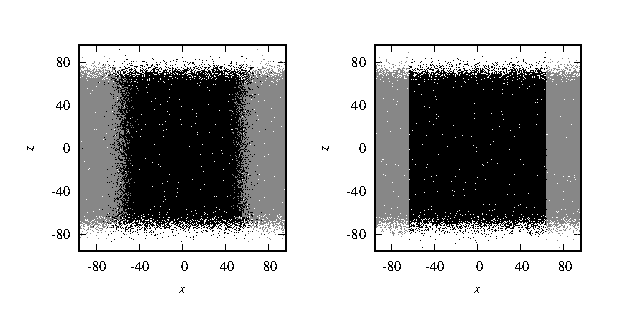
\includegraphics[width = \textwidth]{figures/freeExpansion.eps}
  \caption{\label{freeExpansion}Free expansion of an ideal gas in the $z$
           direction. The system is periodic along the $xy$ plane. On the left,
           the black dots represent particles that were inside the simulation
           box at the start of the computation, and grey dots represent their
           periodic images. On the right, black dots point out the particles
           inside the simulation box at the end of the computation, while grey
           dots mark the positions of particles in other boxes.}
\end{figure}

\section{Initial conditions}

Previously, we have chosen random initial positions, distributed uniformly, for 
the particles; a dangerous choice if we were not dealing with an ideal gas. In 
many systems, particles resist being pushed too close together with great force. 
As you increase the density of particles, you make it more probable for 
particles placed randomly to fall too close to each other. Overlapping particles 
may feel a huge repulsion and shoot off, causing a chain reaction that makes 
your system blow up in the first few steps of a simulation.

A simple solution, apart from reading the initial conditions in from an external 
file, consists in setting particles on the nodes of a crystal lattice and 
letting them reshuffle during the initial stages of the simulation. As an
illustration, include the right header,
\begin{lstlisting}
# include "utils/InitialConditions.cuh"
\end{lstlisting}
and change the inital conditions block to
\begin{lstlisting}
%! codeblock: latticeInitialConditions
  real L = 128;

  %! codeinsert: LJsimulationBox
  {
    auto position
      = particles->getPos(access::location::cpu,
                          access::mode::write);

    auto initial =  initLattice(box.boxSize,
                                numberOfParticles, sc);

    std::copy(initial.begin(), initial.end(), position.begin());
  } //!
%! codeblockend !//
\end{lstlisting}
The ``\texttt{sc}'' parameter in \texttt{initLattice} refers to ``simple
cubic''. Other options are face-centred cubic (\texttt{fcc}), body-centred cubic
(\texttt{bcc}), hexagonal close-packed (\texttt{hcp}), diamond structure
(\texttt{dia}) and the two-dimensional triangular (\texttt{tri}) and square
(\texttt{sq}) lattices. Remember to reset the periodicity
(\texttt{periodicityZ = true}) and size of the box in the $z$ direction.
\begin{comment}
\begin{lstlisting}
%! codeblock: LJsimulationBox
  Box box(make_real3(L, L, L));
  bool periodicityX = true, periodicityY = true,
       periodicityZ = true;
  box.setPeriodicity(periodicityX, periodicityY,
                     periodicityZ); //!
%! codeblockend !//
\end{lstlisting}
\end{comment}

Concerning the velocities, the ideal gas example picked random directions and set
the speeds in such a way that you got the selected energy per particle.
This choice should be fine for our present example, but perhaps you
would later like to experiment imposing an initial sine-shaped velocity profile.
In that event, you could set \texttt{VerletParams.initVelocities} to false and
then write something like this:
\begin{lstlisting}
  {
    auto position
      = particles->getPos(access::location::cpu,
                          access::mode::read);
    auto velocity
      = particles->getVel(access::location::cpu,
                          access::mode::write);

    for(int i = 0; i < numberOfParticles; ++i)
      velocity[i].x
        = sin(2*M_PI*position[i].z/L);
  }
\end{lstlisting}

While we are on the subject of writing your own mathematical functions, I must 
mention that in C++/Cuda you do not write $x^2$ as \texttt{x{\textasciicircum}2} 
or \texttt{x**2}, but rather as \texttt{x*x} or \texttt{pow(x, 2)}.

\section{Interactions}

The final ingredient in our beginner simulations concerns interactions among 
particles. Nothing exciting happens while particles cannot bounce off, repel or 
attract each other. Here we focus on short-range forces, meaning that they fall 
off quicker than the distance between particles squared. If that is the case, 
unless we make the simulation box tiny, particle number $i$ will interact with 
at most one of the periodic copies of particle $j$. The \textit{minimum-image 
convention} states that, when we calculate interactions involving particle 
number $i$, we will neglect all the interactions with periodic images of 
particle number $j$, except perhaps the closest one (see Figure 
\ref{minimum-image_convention}).

\begin{figure}
  \centering
  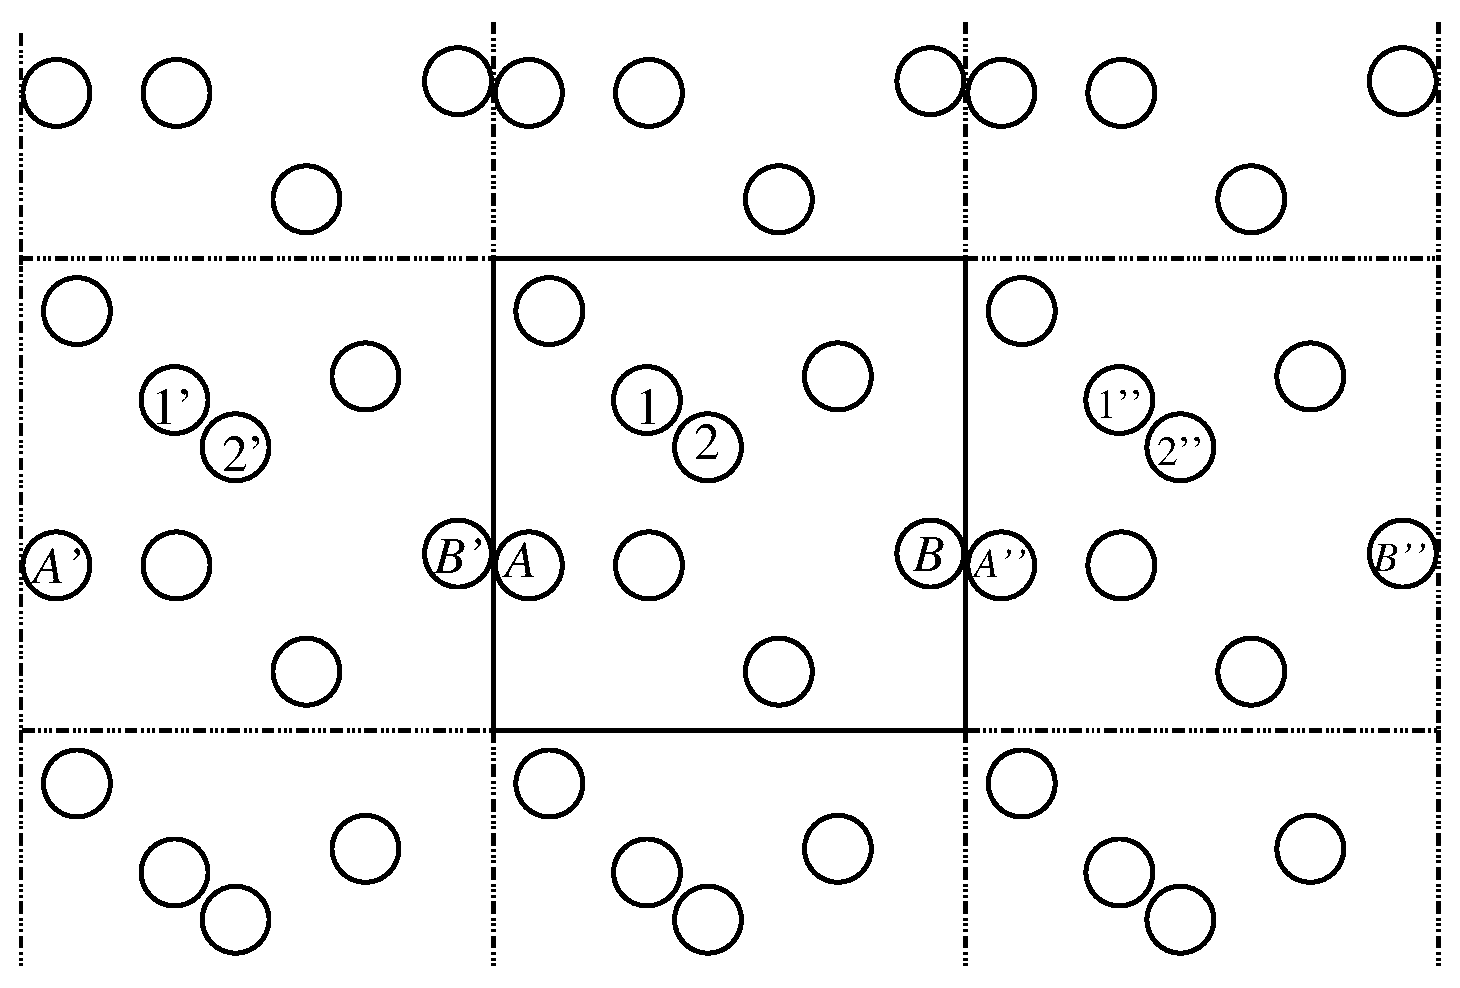
\includegraphics[width = \textwidth]{figures/minimum-image_convention.eps}
  \caption{\label{minimum-image_convention}Particles in a periodic system, with
           a simulation box drawn in solid lines. Particles $1$ and $2$ in the
           box interact with each other, but with none of their periodic images,
           which lie too far away (two of the periodic images of particle $1$
           have been labelled $1'$ and $1''$, and similarly for particle $2$).
           In contrast, particle $A$ does not interact with particle $B$ at the
           other side of the box, but it does interact with an image of $B$
           (labelled $B'$). Similarly $B$ interacts with $A''$.}
\end{figure}

A prototypical example of a molecular dynamics simulation involves spheres 
interacting with each other through a Lennard-Jones potential,
\begin{equation*}
  V(r) = 4\epsilon\left(\left(\frac{\sigma}{r}\right)^{12}
                        - \left(\frac{\sigma}{r}\right)^6\right). 
\end{equation*}
The energy $V$ depends on the distance $r$ between the centres of spheres. If 
the particles come closer than $\sigma$, then they feel a strong repulsion. At
greater distances, they attract each other weakly with a force that falls off
as the sixth power of $r$, in accordance with the law for London dispersion
forces. In the right circumstances, particles may stick together, bonding with
an energy equal to $\epsilon$. Systems with Lennard-Jones interactions represent
neutrally-charged swarms of atoms, such as low-temperature argon, and have been
studied in such great detail that they are used extensively for verifying that
code works correctly and for comparing efficiencies.

A very common speed-up trick sets a cut-off radius (usually at
$r = r_{\mathrm{cut}} = 2.5 \sigma$) beyond which $V(r) = 0$. Some researchers
also shift the potential slightly to avoid the discontinuity in $V$ at
$r = r_{\mathrm{cut}}$.

If you want to incorporate the Lennard-Jones interactions, you have to carry out 
the following three steps:
\begin{enumerate}
  \item Specify the functional form of the interaction.
  \item Create an \textit{interactor}.
  \item Add the \textit{interactor} to the \textit{integrator}.
\end{enumerate}

Take each point in turn, beginning with the potential function. To incorporate
it, we add
\begin{lstlisting}
# include "Interactor/Potential/Potential.cuh"
\end{lstlisting}
to our include list at the beginning of the code file. Fortunately, the
Lennard-Jones potential has already been implemented in UAMMD, so we
only need to specify its parameters.
\begin{lstlisting}
%! codeblock: Lennard-JonesPotential
  auto LJPotential = make_shared<Potential::LJ>(sys);
  {
    Potential::LJ::InputPairParameters LJParams;
    LJParams.epsilon = 1.0;
    LJParams.sigma = 1.0;
    LJParams.cutOff = 2.5*LJParams.sigma;
    LJParams.shift = true;
    LJPotential->setPotParameters(0, 0, LJParams);
  } //!
%! codeblockend !//
\end{lstlisting}
You should find these parameters self-evident with the exception of the first
two zeros in \texttt{setPotParameters}. These indicate that we are setting the
interaction potential among particles of type 0. If we wished to add, for
example, a different type of interaction between particles of type 0 and 1,
then we would have a similar listing ending in something like
\begin{lstlisting}
    LJPotential->setPotParameters(0, 1, LJParams2);
\end{lstlisting}

Step two mentioned creating an ``interactor''. We will use the
\texttt{PairForces} module.
\begin{lstlisting}
# include "Interactor/PairForces.cuh"
\end{lstlisting}

Taking the point of view of a physicist, think of an interactor as an 
\textit{interaction} that the integrator must take into account to calculate the 
motions. We must provide the algorithm for short-ranged forces with the 
information about the simulation box, so that it can calculate interactions 
using the minimum-image convention, as in the first paragraph in the snippet 
below.The new interaction is defined next, using the reference to our system 
(\texttt{particles}), the system (\texttt{sys}), information about the 
simulation box (\texttt{interactionParams}) and, finally, the Lennard-Jones 
potential that we defined above (\texttt{LJPotential}).

\begin{lstlisting}
%! codeblock: Lennard-JonesInteraction
  {
    using LJForces = PairForces<Potential::LJ>;
    LJForces::Parameters interactionParams;
    interactionParams.box = box;

    auto interaction
      = make_shared<LJForces>(particles, sys,
                              interactionParams,
                              LJPotential);

    integrator->addInteractor(interaction);
  } //!
%! codeblockend !//
\end{lstlisting}
The code block ends with step three: adding the interaction to the integrator
with the \texttt{addIntegrator} method.

With this, we have transformed our ideal gas into a system capable of phase
transitions and interfaces. Remember to change the name of the output file to
something more meaningfull, like ``\texttt{Lennard-Jones.dat}''.
\begin{comment}
\begin{lstlisting}
%! codefile: code/Lennard-Jones.cu
# include "uammd.cuh"
# include "utils/InitialConditions.cuh"
# include "Interactor/Potential/Potential.cuh"
# include "Interactor/NeighbourList/CellList.cuh"
# include "Interactor/PairForces.cuh"
# include "Integrator/VerletNVE.cuh"

using namespace uammd;
using std::make_shared;
using std::endl;

int main(int argc, char *argv[]){

  auto sys = make_shared<System>(argc, argv);

  %! codeinsert: particleData

  %! codeinsert: latticeInitialConditions

  %! codeinsert: VerletParams

  %! codeinsert: Verlet

  %! codeinsert: Lennard-JonesPotential

  %! codeinsert: Lennard-JonesInteraction

  std::string outputFile = "Lennard-Jones.dat";
  std::ofstream out(outputFile);

  int numberOfSteps = 1000;
  int printEverynSteps = 100;

  %! codeinsert: integration

  sys->finish();

  return 0;
} //!
%! codeend !//
\end{lstlisting}
\end{comment}
A plot of the final positions after running the program will probably not look
very different from the case for an ideal gas, but calculating the radial
distribution function from this set of our $10^5$ particles reveals a very
obvious spike that you will not find in the case of an ideal gas (see Figure
\ref{Lennard-Jones.rdf}). You can easily remove the Lennard-Jones interaction by
commenting out the \texttt{addInteractor} line to deactivate it.
\begin{lstlisting}
    /* integrator->addInteractor(interaction); */
\end{lstlisting}
The simulation would then generate the plot on the left of Figure
\ref{Lennard-Jones.rdf}.

The radial distribution function measures how the particle distribution around a
typical particle differs on average from that of an ideal gas. In the latter
case, particles distribute uniformly in the volume, but when you activate the
interaction, particles cannot approach each other too closely, so you see that
$g(r) \approx 0$ when $r < \sigma$. Furthermore, particles can stick together,
leading to the subsequent spike. Farther away, the distribution appears as
homogenous as an ideal gas but, as we will see in the chapter on the Langevin
thermostat, more and more peaks appear as you lower the temperature of the
environment.

\begin{figure}
  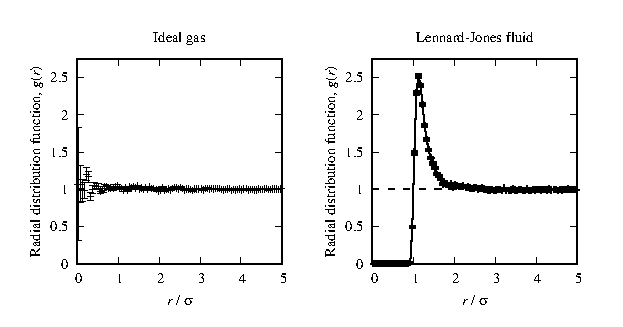
\includegraphics[width = \textwidth]{figures/Lennard-Jones.rdf.eps}
  \caption{\label{Lennard-Jones.rdf}Radial distribution function $g(r)$ for an
           ideal gas (\textit{left}) and a Lennard-Jones fluid (\textit{right}).
           The dashed line represents the theoretical $g(r) = 1$ for an ideal
           gas. Points (with errorbars) present the estimation of $g(r)$
           obtained from the positions in the final step of the simulation
           written in this section.}
\end{figure}

\section{\label{Parameter_files}Parameter files}

Having completed your first interesting simulation, you will want to play with
it. What happens when you change the number of particles? What about the cut-off
radius, or the Lennard-Jones $\epsilon$ and $\sigma$ parameters? You see, now
you can carry out your own virtual experiments. However, having to recompile the
program every single time that you adjust a parameter quickly becomes annoying.
Why not compile the program once and have it read in the parameters from the
command-line or an external file? There are many ways to achieve this, but we
will focus on a neat tool written for UAMMD. You get it for free by inserting
\begin{lstlisting}
# include "utils/InputFile.h"
\end{lstlisting}
at the top of your code. Now let us create a data structure containing a list of
all the parameters that we need to run our simulation.
\begin{lstlisting}
%! codeblock: parameterList
struct InputParameters {
  int numberOfParticles;
  real L;
  real dt;
  real epsilon;
  real sigma;
  real cutOff;
  real particleEnergy;
  std::string outputFile;
  int numberOfSteps;
  int printEverynSteps;
}; //!
%! codeblockend !//
\end{lstlisting}
Next, we ask the program to input the variables from an external file named
\texttt{data.main} and store the values in our data structure. The rest of the
program assigns the parameter values by taking them from the data structure.
To avoid code bloat, we will write a separate function capable of reading in
all the data from the file. We will write the following function before our
\texttt{main}:
\begin{lstlisting}
%! codeblock: readParameterFile
InputParameters readParameterFile(std::shared_ptr<System> sys)
{ //!
%! codeinsert: defaultFile
%! codeinsert: readParameters
%! codeblockend !//
\end{lstlisting}
If the \texttt{data.main} file did not exist when the program was run, we should
create it containing some safe default values.
\begin{lstlisting}
%! codeblock: defaultFile
  if(!std::ifstream("data.main").good()) {
    %! codeinsert: defaultFileMsg
    std::ofstream defaultParameters("data.main");
    %! codeinsert: fileErrorMsg
    defaultParameters<<"numberOfParticles 100000"<<endl;
    defaultParameters<<"boxSize 128"<<endl;
    defaultParameters<<"timeStep 0.01"<<endl;

    /* And so on for all the other parameters ... */
    %! codeinsert: moreDefaultParameters
  } //!
%! codeblockend !//
\end{lstlisting}
\begin{comment}
\begin{lstlisting}
%! codeblock: moreDefaultParameters
    defaultParameters<<"epsilon 1.0"<<endl;
    defaultParameters<<"sigma 1.0"<<endl;
    defaultParameters<<"cutOff 2.5"<<endl;
    defaultParameters<<"particleEnergy 1.0"<<endl;
    defaultParameters<<"outputFile Lennard-Jones.dat"<<endl;
    defaultParameters<<"numberOfSteps 10000"<<endl;
    defaultParameters<<"printEverynSteps 1000"<<endl; //!
%! codeblockend !//
\end{lstlisting}
\end{comment}
To read in the data from the parameter file, we open \texttt{data.main} as an
input file which we will refer to as \texttt{parameterFile}.
\begin{lstlisting}
%! codeblock: readParameters
  InputFile parameterFile("data.main", sys);
  InputParameters params;

  parameterFile.getOption("numberOfParticles",
    InputFile::Required)>>params.numberOfParticles;
  parameterFile.getOption("boxSize",
    InputFile::Required)>>params.L;
  parameterFile.getOption("timeStep",
    InputFile::Required)>>params.dt;

          /* And so on ... */
  %! codeinsert: readMoreParameters

  return params;
} //!
%! codeblockend !//
\end{lstlisting}
\begin{comment}
\begin{lstlisting}
%! codeblock: readMoreParameters
  parameterFile.getOption("epsilon",
    InputFile::Required)>>params.epsilon;
  parameterFile.getOption("sigma",
    InputFile::Required)>>params.sigma;
  parameterFile.getOption("cutOff",
    InputFile::Required)>>params.cutOff;
  parameterFile.getOption("particleEnergy",
    InputFile::Required)>>params.particleEnergy;
  parameterFile.getOption("outputFile",
    InputFile::Required)>>params.outputFile;
  parameterFile.getOption("numberOfSteps",
    InputFile::Required)>>params.numberOfSteps;
  parameterFile.getOption("printEverynSteps",
    InputFile::Required)>>params.printEverynSteps; //!
%! codeblockend !//
\end{lstlisting}
\end{comment}
In the main function, after declaring the System \texttt{sys}, we read in all
the parameter values with
\begin{lstlisting}
%! codeblock: loadParameters
  %! codeinsert: loadParameterMsg
  InputParameters simParams = readParameterFile(sys); //!
%! codeblockend !//
\end{lstlisting}
Whenever we need a parameter value in the remaining code, we just assign it from
the \texttt{simParams} data structure, as in
\begin{lstlisting}
  int numberOfParticles = simParams.numberOfParticles;
  real L = simParams.L;
\end{lstlisting}
and so on.

Running our program for the first time will generate the \texttt{data.main} text
file. Open the file and change the parameters. The next time the program
executes, it will use \texttt{data.main} to set the values for the simulation.

The \texttt{getOption} method was designed to ignore lines beginning with a hash
sign (\#), which you can use to insert comments in your \texttt{data.main} file.
Furthermore, you can define entries as ``Optional'' instead of ``Required''. The
program will continue even if it does not find the option in that file.

Do not use ``\texttt{shell}'' as the name of a parameter.  This reserved word 
provides a neat tool that allows you to execute instructions on the 
command-line. For example, on a Unix-like system you could make a copy of the 
parameter file by writing the following command at the end of the 
\texttt{data.main} file.
\begin{lstlisting}
shell cp data.main LJparameters.dat
\end{lstlisting}
This would create a file called \texttt{LJparameters.dat} containing a copy of 
the values that you ran your simulation with. You could then include a time 
stamp at the end by adding
\begin{lstlisting}
shell echo "# Simulation run on $(date)." >> LJparameters.dat
\end{lstlisting}
UAMMD executes \texttt{shell} commands in the order found in the parameter file.

\section{Logging}

In his ``At Home in the Universe'', John Archibald Wheeler defined an expert as
``someone who knows from his own bitter experience almost all possible mistakes
in his field'' and therefore encouraged researchers to learn how to quickly make
mistakes and fix them. If you intend to write code, accept that you will often
spend more time looking for mistakes than it took you to write the code in the
first place.

The first sign of a problem with your code comes when it doesn't compile. Here 
the compiler error messages and	warnings will help you pinpoint	the mistake. But 
many times, the program will compile fine and do something different from what 
you expected. Before you learn how to use debuggers, you will probably just ask 
the program to print out more information, so that you can track what goes on in 
the different steps.

We \textit{could} use \texttt{cout} to print this information onto the screen, 
but UAMMD includes a convenient function that allows you to print messages with 
different priorities. To inform the user that the program will read the 
parameter file, write
\begin{lstlisting}
%! codeblock: loadParameterMsg
  sys->log<System::MESSAGE>("Reading parameters from data.main."); //!
%! codeblockend !//
\end{lstlisting}
just before you call the \texttt{readParameterFile} function in \texttt{main}.

Suppose the \texttt{data.main} file did not exist. Then we would issue a warning
saying that the program has created this file with a set of default values.
\begin{lstlisting}
%! codeblock: defaultFileMsg
    sys->log<System::WARNING>("File data.main not found. Creating file with default values."); //!
%! codeblockend !//
\end{lstlisting}
What if the operating system did not allow the program to write to the directory
and the file was not created? That would prove catastrophic for the subsequent
program. A \textit{CRITICAL} error message would explain the error and stop the
program.
\begin{lstlisting}
%! codeblock: fileErrorMsg
    if(not defaultParameters.is_open()) {
      sys->log<System::CRITICAL>("Unable to create data.main file. Halting program.");
      exit(-1);
    } //!
%! codeblockend !//
\end{lstlisting}
would exit the program if the file was not open. The UAMMD System provides a
whole set of message types listed here in decreasing order of priority:
\texttt{CRITICAL}, \texttt{ERROR}, \texttt{EXCEPTION}, \texttt{WARNING},
\texttt{MESSAGE}, \texttt{STDERR}, \texttt{STDOUT}, \texttt{DEBUG},
\texttt{DEBUG1}, \texttt{DEBUG2}, \texttt{DEBUG3}, \texttt{DEBUG4},
\texttt{DEBUG5}, \texttt{DEBUG6}, \texttt{DEBUG7}. By default all messages
with priority above DEBUG will be printed.

Use the different levels of debugging to specify what your code is doing at 
different points. The compiler will ignore these messages, but whenever you have 
to deal with a problem, you can activate them. Add the option 
\texttt{-DMAXLOGLEVEL=7} to the command-line options when you compile, and your 
program will now print DEBUG messages. If you increase the level to 8, you will 
also get the DEBUG1 messages. You get the idea.

In a single chapter, we have converted a ``Hello, World!'' program into a 
fully-functional Lennard-Jones fluid simulator. If you enjoyed the recipe and
would like to enlarge your repertoire of cooking utensils, head on to chapter 2,
where we will encounter new interactions, such as bonds and external fields.

\begin{comment}
List of programs written in this chapter:

%! codeblock: codelist
* `minimal.cu`: A minimal UAMMD program that only prints a Hello message and
  then exits.
* `freeExpansion.cu`: Ideal gas expanding freely in the vertical direction with
  periodic boundary conditions in the other two directions.
* `Lennard-Jones.cu`: Particles in a periodic box interacting through a
  Lennard-Jones potential.
* `superLennard-Jones.cu`: Improved Lennard-Jones system with logging and
  external parameter file.
%! codeblockend

Final version of the Lennard-Jones simulation program:
%! codefile: code/superLennard-Jones.cu
# include "uammd.cuh"
# include "utils/InputFile.h"
# include "utils/InitialConditions.cuh"
# include "Interactor/Potential/Potential.cuh"
# include "Interactor/NeighbourList/CellList.cuh"
# include "Interactor/PairForces.cuh"
# include "Integrator/VerletNVE.cuh"

using namespace uammd;
using std::make_shared;
using std::endl;

%! codeinsert: parameterList

%! codeinsert: readParameterFile

int main(int argc, char *argv[]){

  auto sys = make_shared<System>(argc, argv);

  %! codeinsert: loadParameters

  int numberOfParticles = simParams.numberOfParticles;
  auto particles
    = make_shared<ParticleData>(numberOfParticles, sys);

  real L = simParams.L;

  %! codeinsert: LJsimulationBox
  {
    auto position
      = particles->getPos(access::location::cpu,
                          access::mode::write);

    auto initial =  initLattice(box.boxSize,
                                numberOfParticles, sc);

    std::copy(initial.begin(), initial.end(), position.begin());
  }

  using Verlet = VerletNVE;
  Verlet::Parameters VerletParams;
  VerletParams.dt = simParams.dt;
  VerletParams.initVelocities = true;
  VerletParams.energy = simParams.particleEnergy;

  %! codeinsert: Verlet

  auto LJPotential = make_shared<Potential::LJ>(sys);
  {
    Potential::LJ::InputPairParameters LJParams;
    LJParams.epsilon = simParams.epsilon;
    LJParams.sigma = simParams.sigma;
    LJParams.cutOff = simParams.cutOff;
    LJParams.shift = true;
    LJPotential->setPotParameters(0, 0, LJParams);
  }

  %! codeinsert: Lennard-JonesInteraction

  std::string outputFile = simParams.outputFile;
  std::ofstream out(outputFile);

  int numberOfSteps = simParams.numberOfSteps;
  int printEverynSteps = simParams.printEverynSteps;

  %! codeinsert: integration

  sys->finish();

  return 0;
}
%! codeend

\end{comment}


\chapter{Unleash your own potential}

You can only have so much fun playing with a Lennard-Jones simulation. Changing
the parameter values and then looking for differences in your plots gets old
fast. If you have made it this far, you want more. You imagine molecules, or
larger structures. Perhaps you would like to simulate billowing smoke, sloshing
water, or planets orbiting a star. All in good time.

Whatever your final aim, you need new interactions, and this chapter contains a
good collection of them.

\section{Harmonic bonds}

The simplest permanent link between particles in UAMMD has to be the harmonic
bond. Think of it as an invisible linear spring connecting two particles. As
long as they remain at the equilibrium distance $r_0$, they exert no force on
each other, but when you stretch their separation $r$ they pull back. The
potential function for this bond, then, equals
\begin{equation*}
  V(r) = \frac{1}{2}\ k\ (r - r_0)^2,
\end{equation*}
where the spring constant $k$ quantifies the bond rigidity.

Including bonds presents no difficulties from the point of view of UAMMD code,
as the code resembles the lines we wrote for the Lennard-Jones interaction.
\begin{lstlisting}
\end{lstlisting}
The difficulty arises from the need to specify which particles are linked.

\section{Alternative types of bonds}

FENE

Fixed bonds

Angular bonds

Torsional bonds

\section{External fields}

\section{Other potentials (DPD, SPH)}

\section{Defining your own potentials}

Bond potentials

Pair interactions


\chapter{Macroscopic quantities}

\section{Energy}

\section{Temperature}

\section{Pressure}


\chapter{The Langevin thermostat}

seeding the PRNG


\chapter{Long-range interactions}

\chapter{Hydrodynamics}

SPH and DPD

\chapter{Advanced topics}

\end{document}

%! codefile: Makefile
all: tangle weave

tangle:
	txt2tangle uammd_intro.tex
	for file in `ls chapters/*.tex`; do txt2tangle $$file; done

weave:
	latex uammd_intro.tex
	dvips uammd_intro.dvi
	ps2pdf uammd_intro.ps
%! codeend

%! codefile: README.md
# A Painless Introduction to Programming UAMMD Modules

UAMMD stands for **Universally Adaptable Multiscale Molecular Dynamics**. You
can find the project at:

[https://github.com/RaulPPelaez/UAMMD]

%! codeinsert: OnUAMMD src: chapters/introduction.tex

I have copied the entire example programs discussed in the main text into the
**code** folder.

%! codeend

%! codefile: code/README.md
# Example programs

## Introduction

  %! codeinsert: codelist src: chapters/introduction.tex

## Our first UAMMD simulation

  %! codeinsert: codelist src: chapters/first_simulation.tex

## Unleash your own potential

  %! codeinsert: codelist src: chapters/potentials.tex
%! codeend
